\label{Proposed}

Health RS plays an essential role in food, diet, and physical activity
recommendation, and RS research is growing fast, especially in the e-commerce
sector \cite{Tran2021b}. However, the RNN prediction solutions
like Wang et al. \cite{Wang} and PREMIER \cite{Bhoi2021} only incorporate past diagnoses and past
procedures. Our proposed solution for this study is to use the vast amount of
data in EHR like MIMIC in the RS.  The following describes our proposed ways of
tackling the objectives.


\subsubsection{
    Tackling cold start issues for new patients
}

The more features the system contains, the more it can handle cold start issues
for new patients with little data. For example, if the system is trained on the
age, diagnoses and procedures and a new user only has the first two, the system
should be capable of recommending the right medicine. 

\subsubsection{
Finding the best Model
}
After splitting the dataset into a training set and a
testing set, we want to find the best model that
achieves the highest scores using libraries like Pytorch
to build our model. We could also compare then replace
our model with sequence modelling techniques like
transformers to see if the system improves. For example,
PREMIER \cite{Bhoi2021} replaced the RNN with BERT, and
their system improved from 78\% to 82\% accuracy.

\subsubsection{
    Preventing adverse side effects from recommendations
}
We can aggregate the EHR dataset with a drug interactions dataset containing
information about a specific medication and its effects and conflicts with
other drugs. This combination ensures that any recommended medicine does not
cause harm or damaging side effects to any patients.
PREMIER \cite{Bhoi2021} combined the MIMIC dataset with a
Drug interactions dataset to check the final recommended
results.

\subsubsection{
    Selecting the best features from the dataset
}
Choosing the best features from the EHR dataset helps us build an efficient
model. Our goal is to determine which data hold value for increasing accurate
predictions. For example, most systems only make use of
diagnoses and procedures. We would like to check whether
demographics and other health-related data like blood
pressure could affect performance.

\section{Testing and Evaluation}

\label{Testing}

\subsection{
The Dataset 
}


The MIMIC (Medical Information Mart for Intensive Care) is a publicly
available EHR dataset under the registration of the university of MIT
containing data from patients admitted to the critical care units of the Beth
Israel Deaconess Medical Center \cite{Johnson2016}.
Several RS use such datasets like LEAP, PREMIER and Wang
et al.'s system \cite{Wang}. 

There are four versions of this database, and after applying, we have been
given access to MIMIC III and MIMIC IV. The third version contains twenty-six
tables, over 40,000 patient records (excluding people under 16), and 53,423
visits between 2001 and 2012. Each patient is de-identified and anonymised and
contains medical intake, chart events, ICU date stays, demographics, doctor's
notes and more. On average, each patient has around 2.68 visits, and table \ref{age}
shows some statistics about the dataset, and figure \ref{statistics} shows the age
distribution of the patients. People over 90 are grouped. Each patient is
identified with a patient ID, used throughout the tables. Diagnosis, Procedures
are encoded using international standards such as ICD-9 and ATC classification .

\begin{figure}[h]
    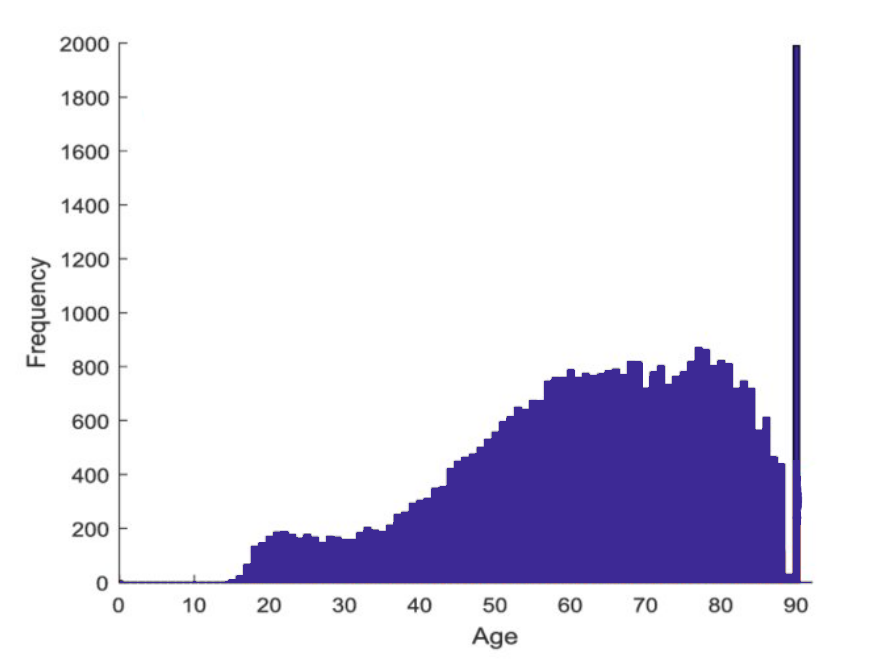
\includegraphics[width=8.5cm, height = 6cm]{ageDistribution.png}
    \caption{Age Distribution of MIMIC III}
    \label{age}
\end{figure}


\begin{table}[h]

    \caption{MIMIC III Statistics.}
    \label{statistics}
\begin{center}
\begin{tabular}{ | c | c | }
    \hline
 Number of patients     & 46520 \\ 
    \hline
 Number of Diagnoses    & 14567 \\  
    \hline
 Number of Procedures   & 3882  \\
    \hline
 Number of Medicine     & 4204  \\
    \hline
\end{tabular}
\end{center}

    \end{table}


\subsection{Evaluation Methodology}

There are three main things to test for evaluating the RS; performance,
accuracy scores and drug interactions tests. These three measures will
ensure that our system would recommend good medicine as fast as possible
whilst also ensuring the patient's safety. We will also compare our
system's safety with other RS using standard drug
interactions metrics. We could also package the system in
an application and present sample use cases to
demonstrate our system. 


\subsection{Evaluation Metrics}

We will split the dataset into training, testing, and validation sets
to calculate additional evaluation metrics such as the F1 score,
precision,Jaccard, Root-mean-square deviation, and Mean Absolute Errors. Doing so
will allow us to compare our system with existing systems that use the
MIMIC dataset. 

